\let\textcircled=\pgftextcircled
\chapter{Theory}
\label{chap:theory}

\initial{T}his is the theory chapter.

%=======
\begin{easylist}[itemize]
\ListProperties(Style*=-- , FinalMark={)}, Margin=0.5cm)
& Give an overview of the fundamental forces and particles.
& Discuss the Standard Model in detail, emphasising certain aspects as they relate to dark matter and the Higgs field (and boson).
& Briefly recap dark matter, referencing descriptions in introduction.
& Discuss the theory behind combined Higgs to inv.: only \acrshort{sm} process in which Higgs decays invisibly is $\PH \rightarrow \PZ\PZ \rightarrow 4\nu$ with branching ratio of 0.1\,\%~\cite{Heinemeyer:1559921}, whilst the current observed experimental limit is 19\,\% from CMS~\cite{Sirunyan:2018owy} and 26\,\% from \acrshort{atlas}~\cite{Aaboud:2019rtt}. If new, invisible particles couple to Higgs, branching ratio will be enhanced. Constraining \BR can also exclude some dark matter models.
& Discuss the theory behind the semi-visible jets analysis (main sources from Refs.~\cite{Cohen:2015toa,Cohen:2017pzm}): strongly interacting dark sector in Hidden Valley scenario with a portal to the visible sector. Mentioning dark quarks \Pqdark, dark confinement scale \lamDark, dark hadronisation and decay, running coupling \aDark, etc.
& Explain some of the phenomenological/experimental event characteristics that overlap with both analyses, i.e., what a jet is, and maybe energy sums like \ptmiss, \HT, \htmiss, etc.
\end{easylist}


\section{The standard model of particle physics}
\label{sec:standardmodel}

% Check Lancaster and other summer school notes (Postgraduate and CMS courses/ folder)


\section{Limitations of the standard model}
\label{sec:sm_limitations}

% Check Lancaster and other summer school notes for other limitations, specifically referencing things that can tie into dark matter


\section{Theoretical motivations for, and descriptions of, dark matter}
\label{sec:dark_matter}

% DON'T RENDER
\iffalse

% Will probably be referring to things from introduction section. Try to just give overview there and describe the nitty-gritty here
Dark matter was thought to be created in the hot, early universe when the thermal background allowed its spontaneous pair production. When the universe expanded and cooled, a thermal freeze out occurred: the average temperature became too low to allow significant production \cite{Baldes:2017gzw}. Matter became further separated and the dark matter annihilation rate decreased, leaving a ``thermal relic". These remaining particles were attracted via gravity, the only known force by which dark matter interacts. They formed filaments throughout the universe, and the potential wells they induced allowed the progenitors of galaxies to form within.

% Taken directly from my lab book. Tidy up and improve
\begin{easylist}[itemize]
\ListProperties(Style*=-- , FinalMark={)})

& It is thought that dark matter was produced thermally in the early universe (when it was hot and therefore easier to create heavy particles). Dark matter particles could (and did) annihilate, but as the universe expanded and cooled the dark matter became more diffuse. They didn't annihilate as often and the dark matter we see today is a "thermal relic" and is what's left over. Some models suggest the parameter $x = m_{\mathrm{DM}}/T \sim 20$ at freeze out. \cite{Lisanti:2016jxe} 

& The current leading dark matter candidate is a WIMP (Weakly Interacting Massive Particle), possibly a neutral supersymmetric particle (neutralino) like a higgsino, photino, zino, etc. One of the motivations for WIMPs are that, using the current values of the dark matter density in the universe and approximations for the annihilation cross section, dark matter could self-interact at the electroweak scale to produce Standard Model particles. \cite{Kamionkowski:1997zb} As the EW scale can be readily accessed at colliders like the LHC, we could detect DM signatures via pair production then annihilation or indirect searches via solely annihilation.

& WIMP annihilation could produce two showers of quarks, which would normally be observed as pions and high energy photons (like gamma rays). The photons may be of a continuum -- from hadronisation and radiation of the decay products of annihilation -- or contain features (internal radiation from the propagator in the interaction or from loop-level processes).

& Because WIMPs are stable (at least on the timescale of the current age of the Universe), they wouldn't decay into other particles when produced from accelerator collisions. So you would detect them (indirectly) by looking for MET and by looking for visible particles recoiling against the WIMPs.

& The mediator (force-carrying particle, like the gauge bosons) for dark matter -- between dark matter particles or the dark matter-Standard Model particle interactions -- may be a scalar (spin-0, like the Higgs boson) or pseudoscalar (reverses parity under a Lorentz transformation, like the pion) boson. [Support] for a pseudoscalar over a scalar mediator comes from the Feynman diagrams for DM annihilation into, e.g., $b$-quarks. With a scalar mediator, the vertex factors and the propagator term lead to cancellations in the cross section equation in the low-velocity limit.

& The mediator for dark matter may be heavier than the dark matter particle itself (like with the $W^{\pm}$ and $Z$ bosons being heavier than most of the particles they mediate), maybe 2x heavier or more so than the DM particle. The mediator could decay via DM pair production, so it makes sense that it would be at least twice as heavy.

& There's no consensus on whether dark matter is fermionic or bosonic. If fermionic, it may be either a Dirac fermion (particle is distinct from its antiparticle, like the electron and positron) or Majorana fermion (particle is the same as its antiparticle, like the neutrino is \underline{suspected} to be). If it were Majorana, dark matter could annihilate with itself, making discoveries via indirect searches more likely.

& At the LHC, monojets are used most prominently to look for dark matter particles. But multijet plus \etmiss might provide better sensitivity and constraints (particularly if the mediator is pseudoscalar).

& \underline{Many} dark matter candidates include a few supersymmetric particles (the neutralino being the most widely studied), sterile neutrinos \cite{doi:10.1142/S0218301313300191}, axions, Kaluza-Klein states \cite{Han:1998sg} (which are excitations of Standard Model fields in extra dimensions), etc.

& The different aspects of dark matter searches: indirect (annihilation), direct (scattering from SM particles), and collider (production). Try to find/make a good image that showcases this (Feynman diagram with arrows for each type of detection).

& Some good results showcasing dark matter masses and that of its mediator from different analyses and decay channels are at \cite{CMS-DP-2016-057}. Particularly figures 4 and 6, which I used in my poster for the PGR conference.

& LUX (Large Underground Xenon experiment) and LZ (LUX-Zeplin) are direct detection experiments that search explicitly for WIMP dark matter. LUX uses an underground liquid xenon tank to detect WIMPs interacting with ordinary matter, the scattering producing photons and electrons of specific energies. LZ is a collaboration between the LUX and ZEPLIN groups, and will have a highly-sensitive WIMP detector over a large range of masses, once completed.

\end{easylist}


% Taken directly from my lab book. Tidy up and improve. Look through these papers to see which ones give compelling interpretations and motivation for dark matter
Papers to look at regarding SUSY and dark matter:

\begin{easylist}[itemize]
\ListProperties(Style*=, FinalMark={)})
& \cite{dmsearcheslhc2015}
& \cite{dmbenchmarkearlylhcrun2}
& \cite{CMS-PAS-EXO-12-055}
& \cite{Martin:1997ns}
& \cite{CMS-PAS-SUS-15-005}
& \cite{Aitchison:2005cf}
& \cite{Ellis:2002mx}
& \cite{Murayama:2007ek}
& \cite{Peskin:2007nk}
& \cite{Goodman:2010ku}
& \cite{PhysRevLett.115.181802}
& \cite{CMS:2016pod}
& \cite{Bertone:2004pz}
\end{easylist}

\fi


\subsection{Measuring the branching ratio for the invisible decays of the Higgs boson}
\label{subsec:theory_higgs_to_inv}

% Can pull from Section 37 in my lab book, as well as all the talk I've given (Presentations and talks/ folder, my IOP one is a good starting point)


\subsection{Searches for semi-visible jets}
\label{subsec:theory_svj}

% Can pull from Section 14 and Section 35 of my lab book, and all the talks I and other people from the team have given (Presentations and talks/ folder, also Other peoples/ subdirectory)

\begin{figure}[htbp]
\centering
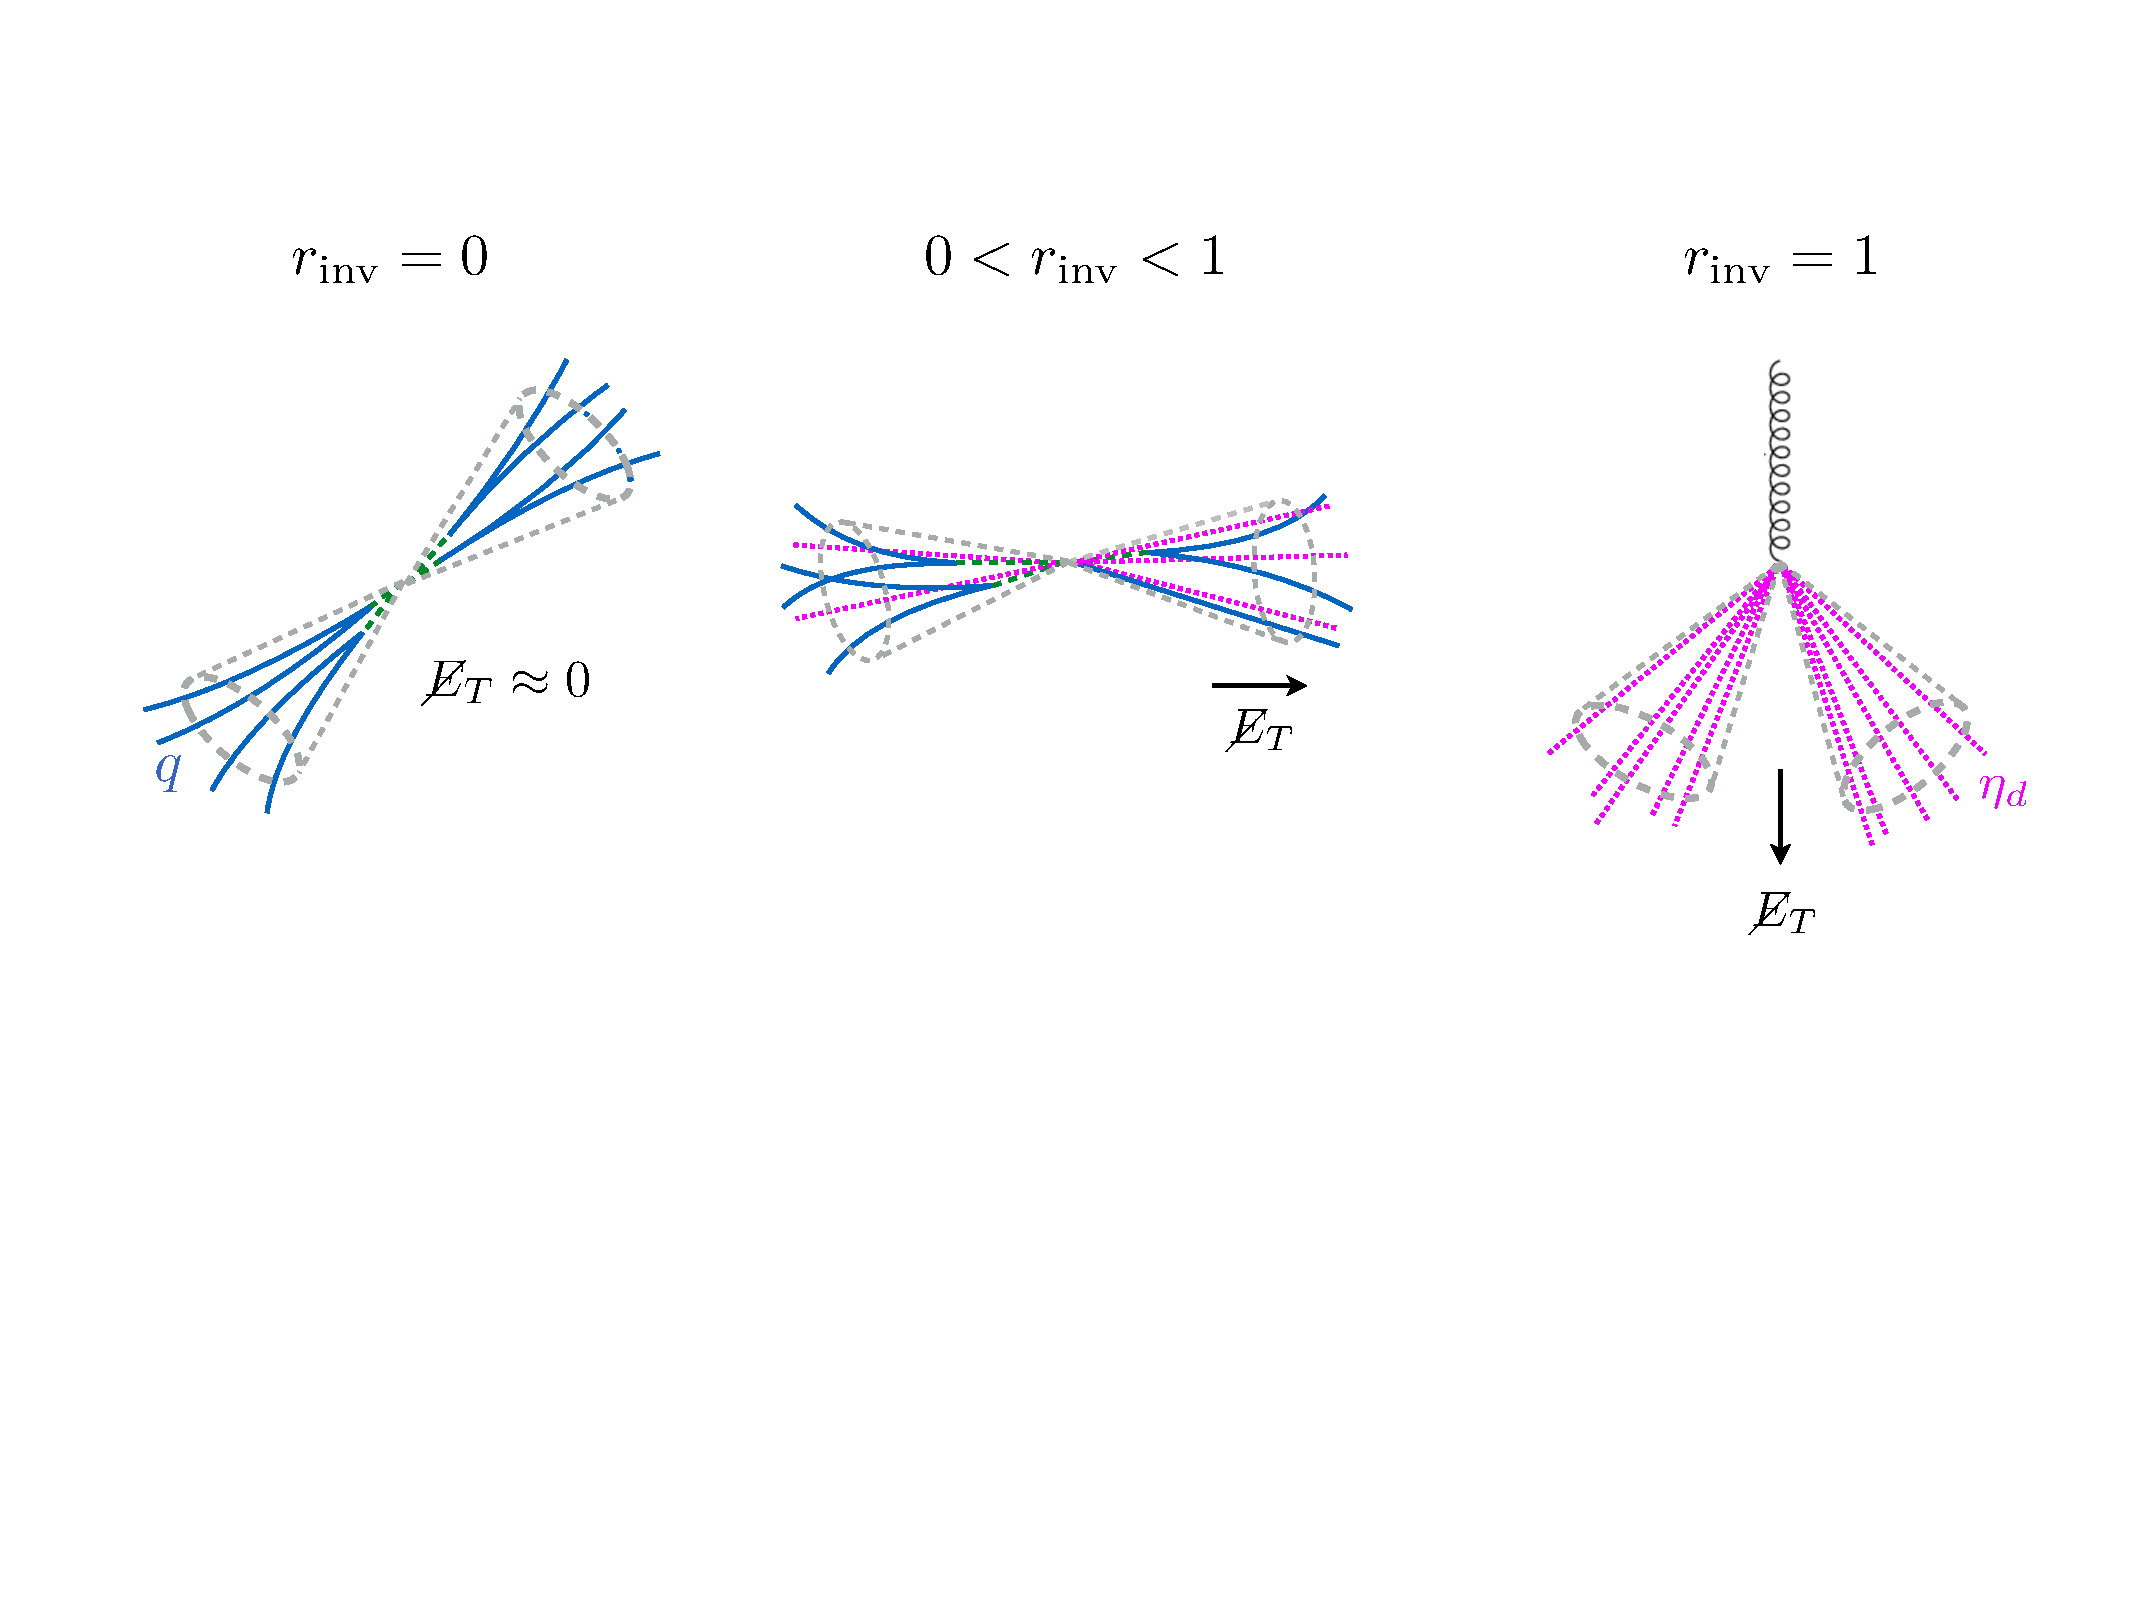
\includegraphics[width=0.85\textwidth]{figures/svj/metfigure.pdf}
\caption[The typical direction of the missing transverse energy relative to the semi-visible jets as a function of the invisible fraction \rinv]{The typical direction of the missing transverse energy \ETslash\xspace (or \ptmiss) relative to the semi-visible jets as a function of their invisible fraction \rinv \cite{Cohen:2017pzm}.}
\label{fig:theory_svj_met_dir}
\end{figure}

\begin{figure}[htbp]
    \centering
    \begin{subfigure}[c]{0.45\textwidth}
    \centering
        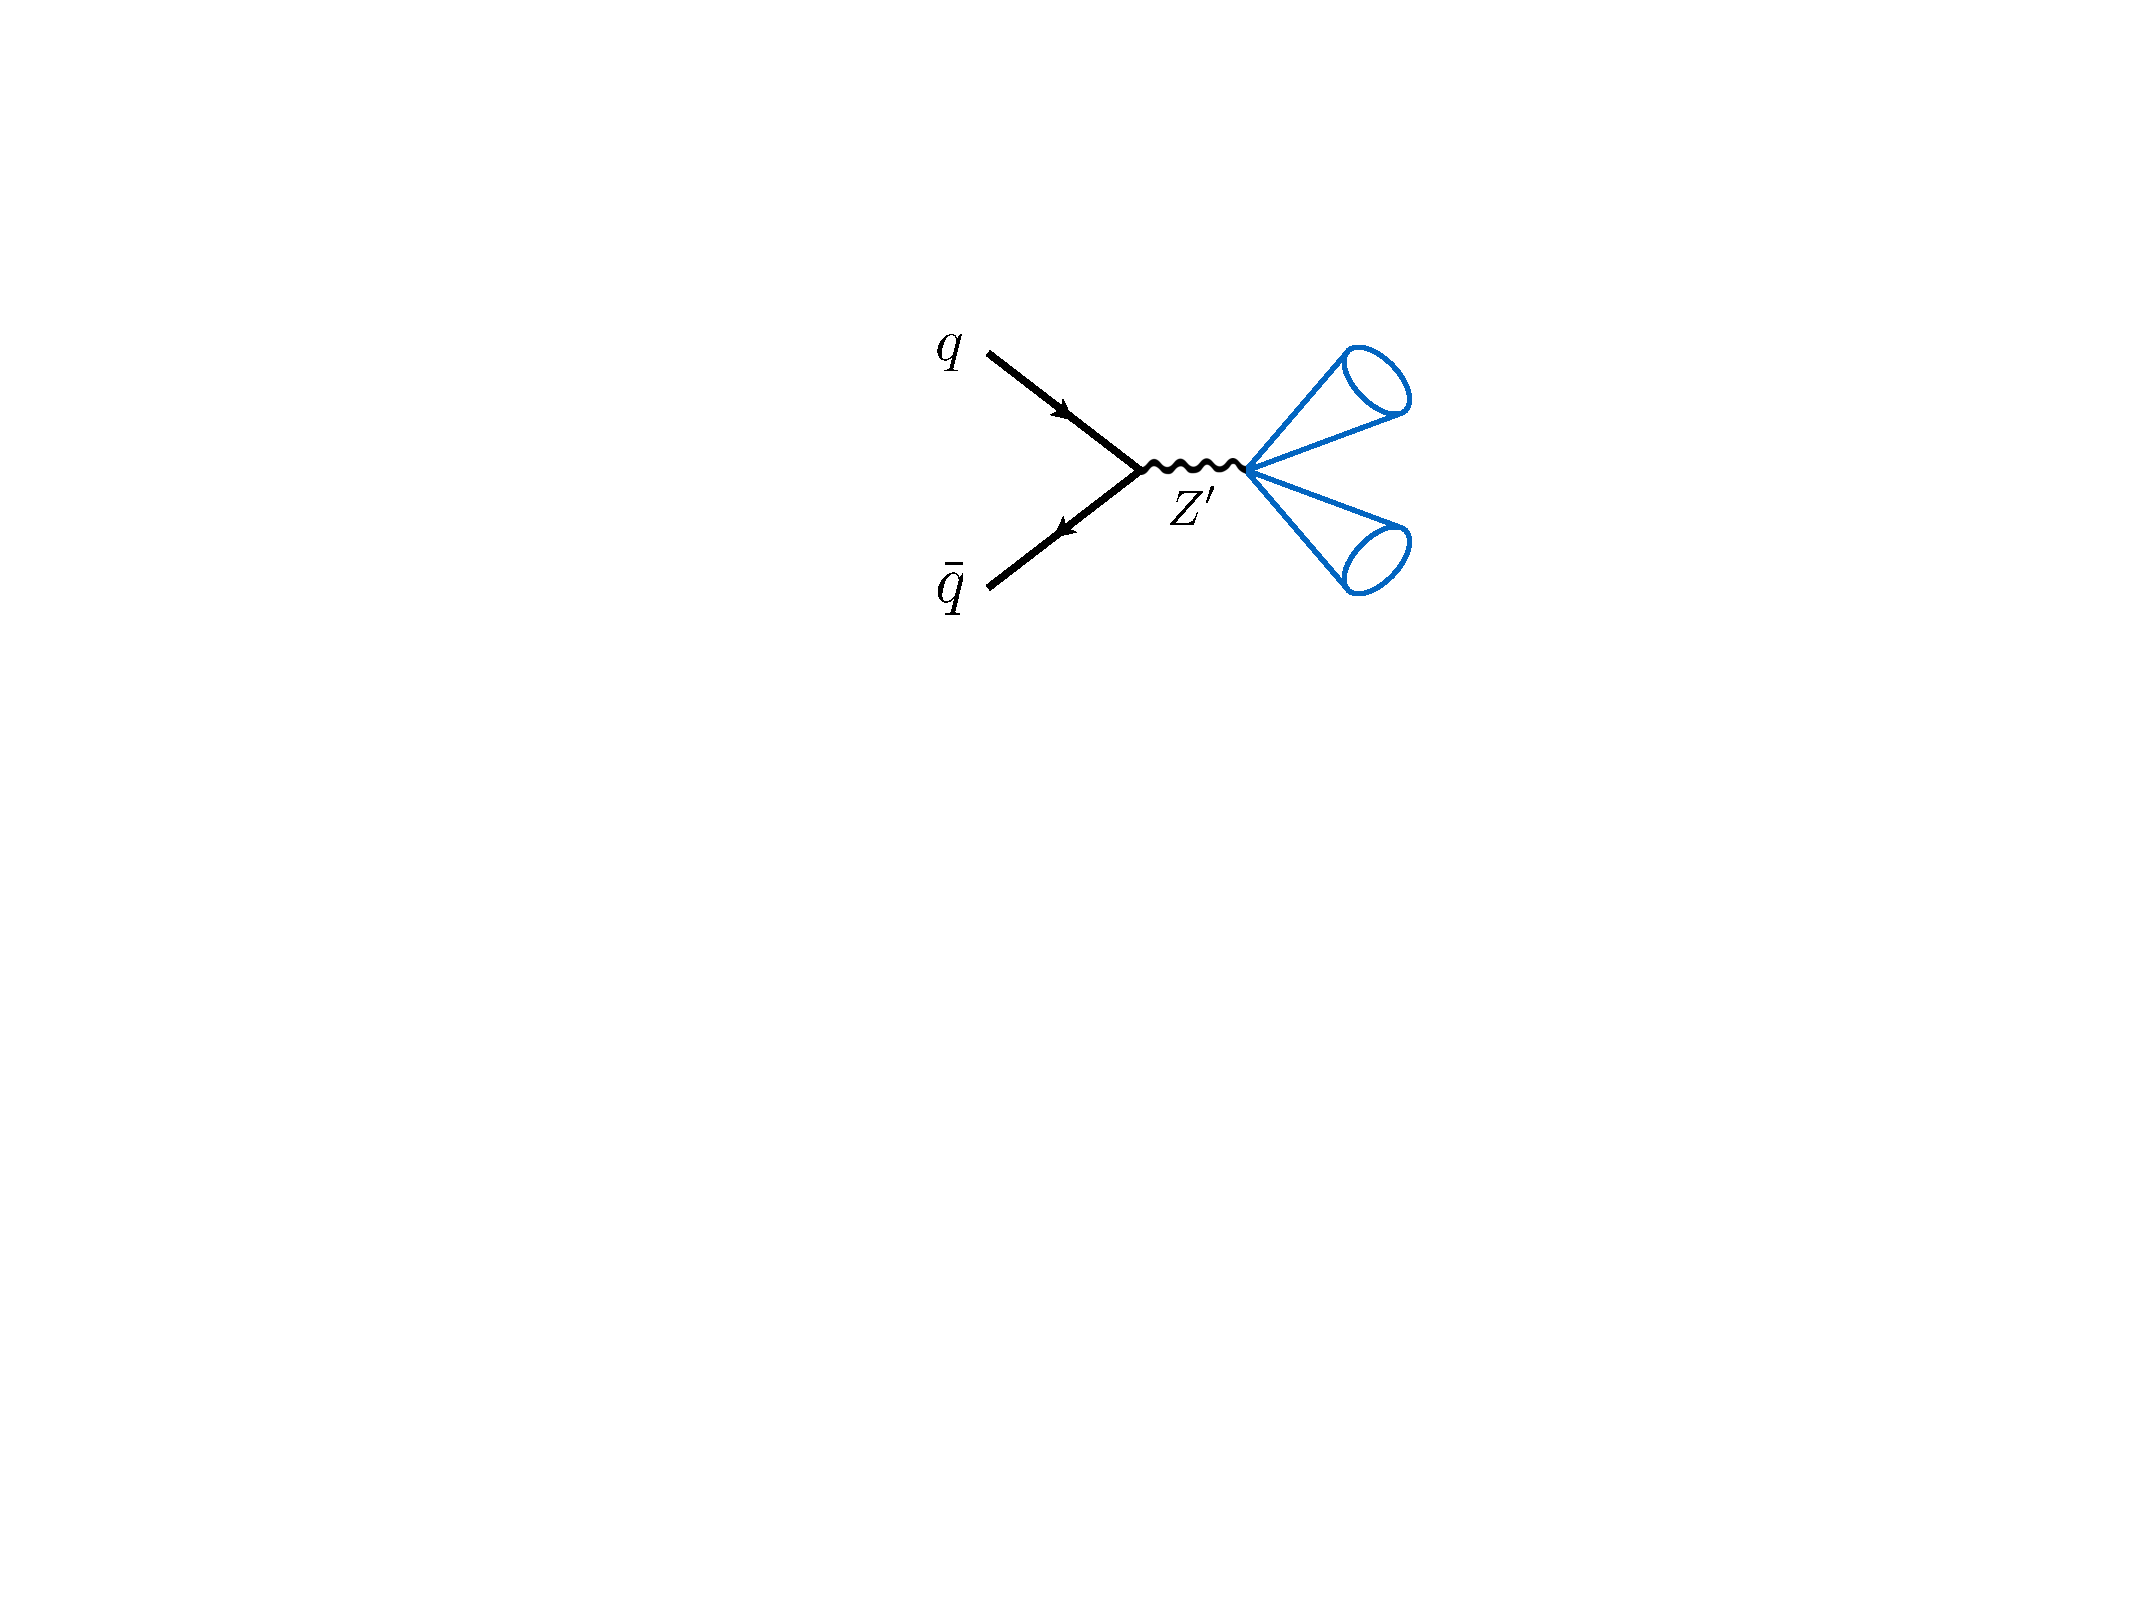
\includegraphics[width=0.7\textwidth]{figures/svj/portals_s.pdf}
        \caption{\schannel}
    \end{subfigure}
    \hfill
    \begin{subfigure}[c]{0.45\textwidth}
    \centering
        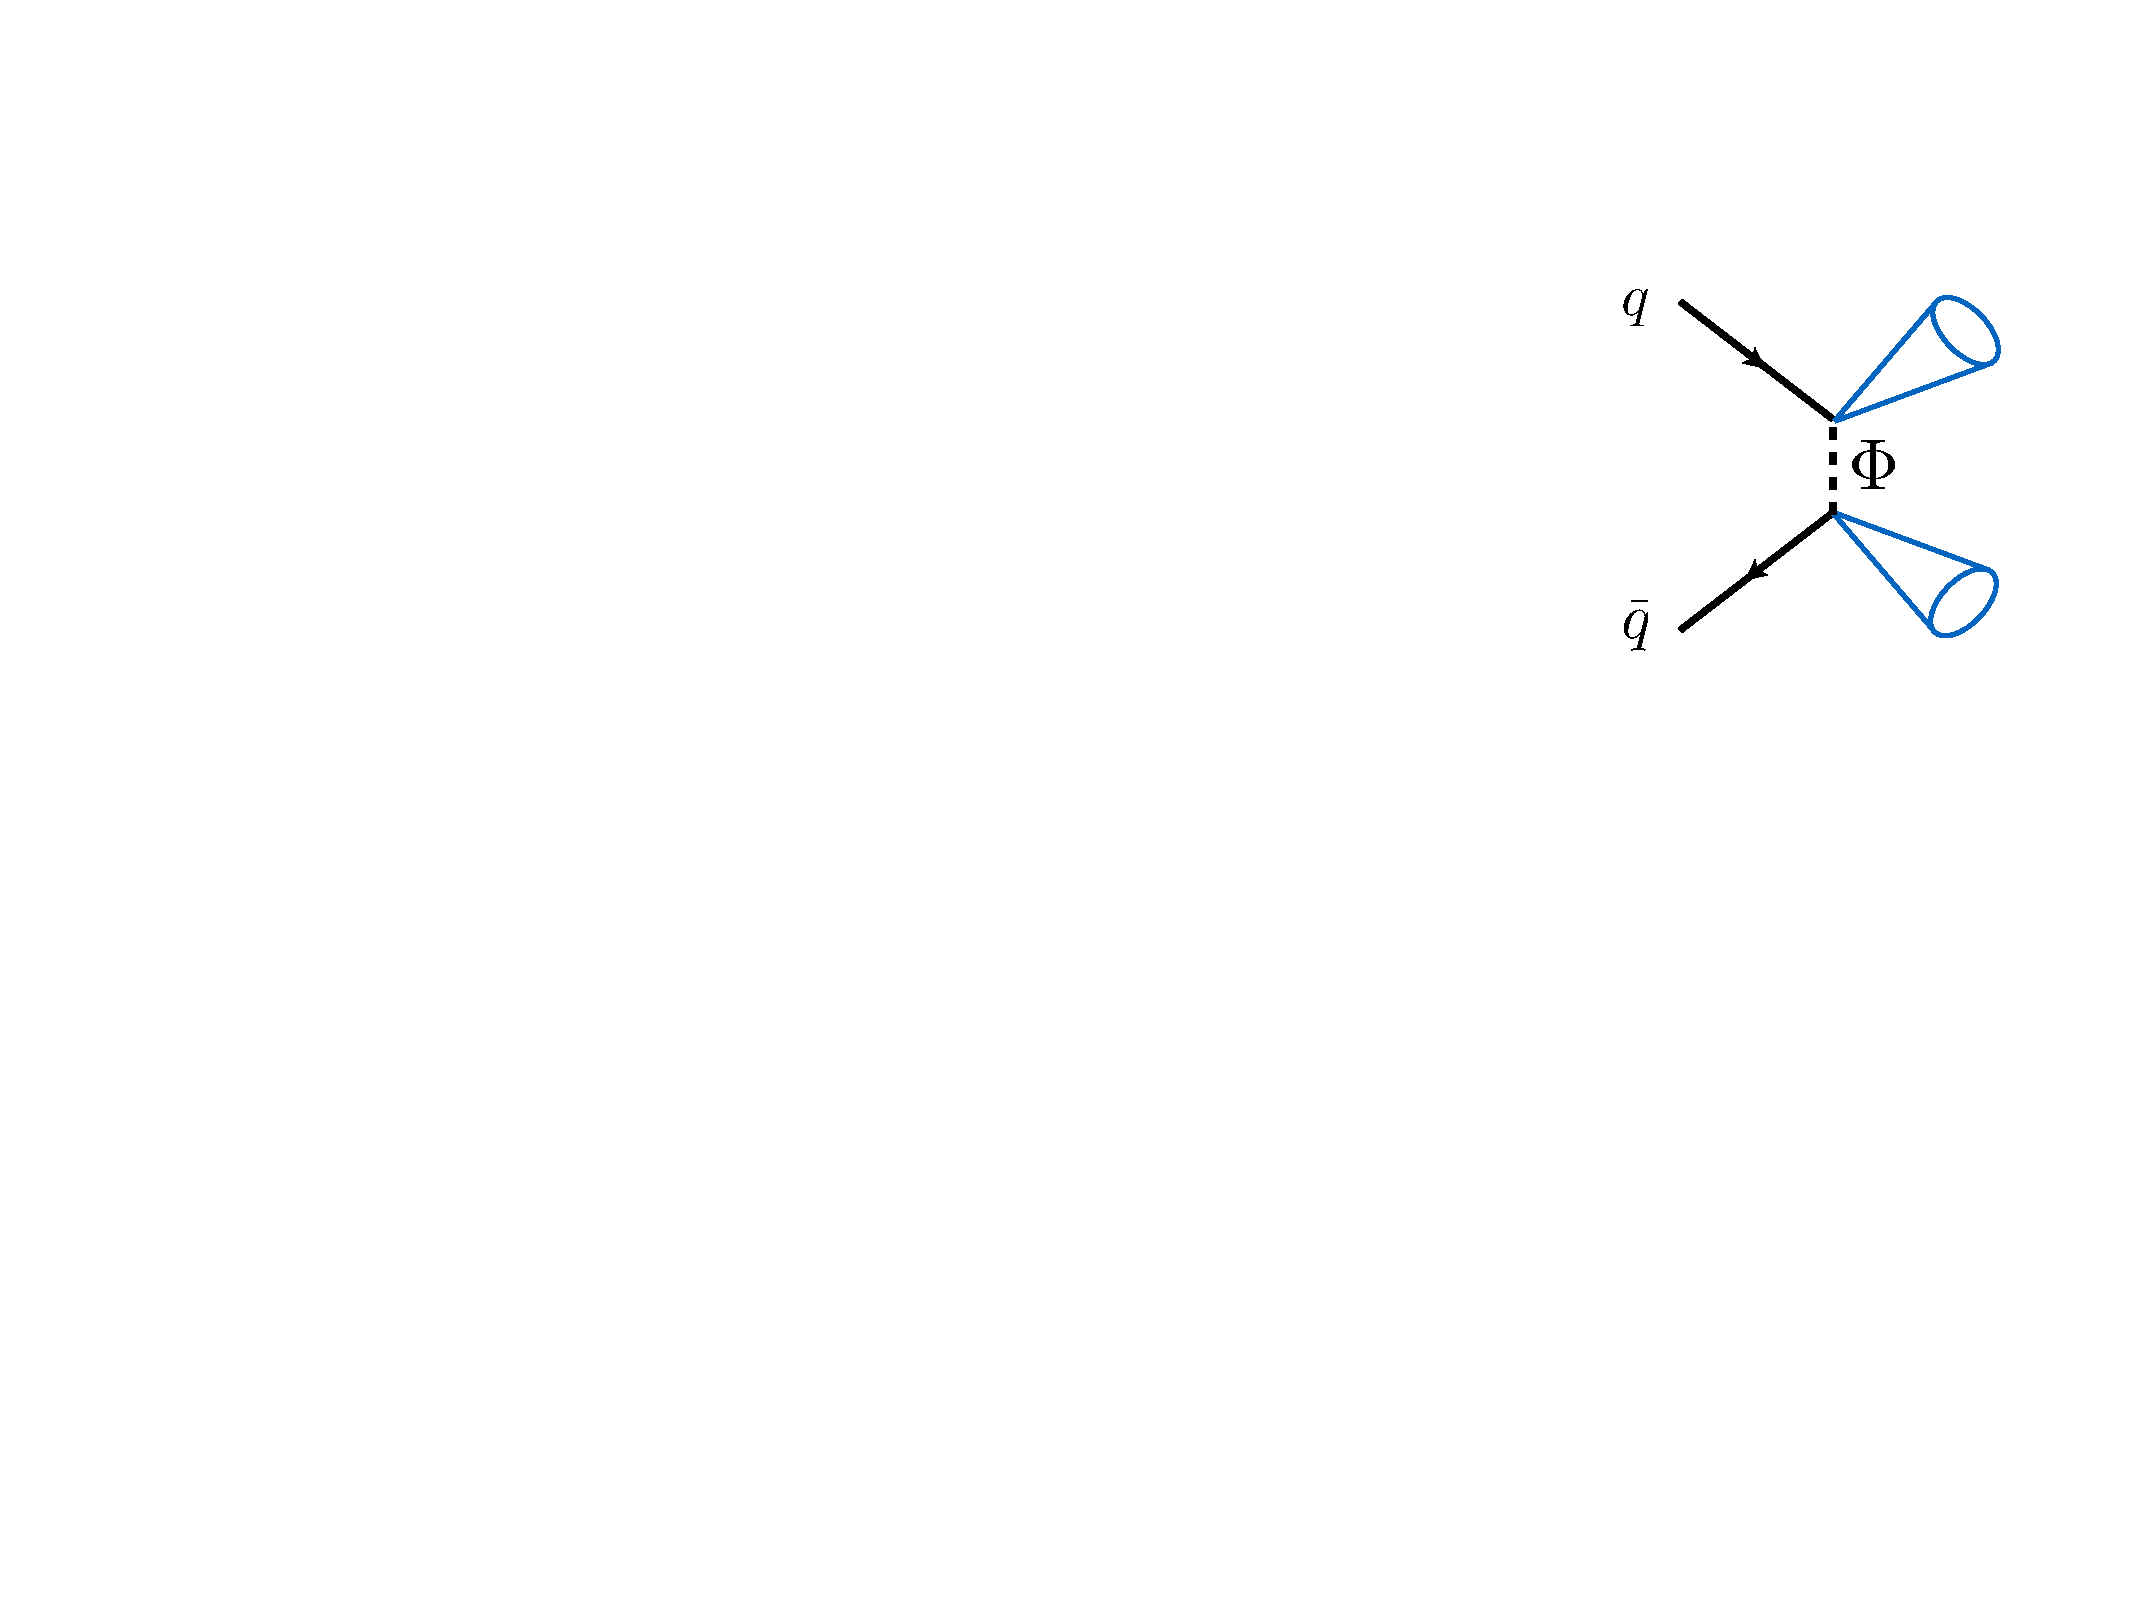
\includegraphics[width=0.7\textwidth]{figures/svj/portals_t.pdf}
        \caption{\tchannel}
    \end{subfigure}
\caption[Example Feynman diagrams for the two main production modes of semi-visible jets. A \PZprime  boson mediates the \schannel process while a bifundamental $\Phi$ mediates the \tchannel process]{Example Feynman diagrams for the two main production modes of semi-visible jets \cite{Cohen:2017pzm}. A \PZprime  boson mediates the \schannel process while a bifundamental $\Phi$ mediates the \tchannel process.}
\label{fig:theory_svj_portals}
\end{figure}

\begin{figure}[htbp]
\centering
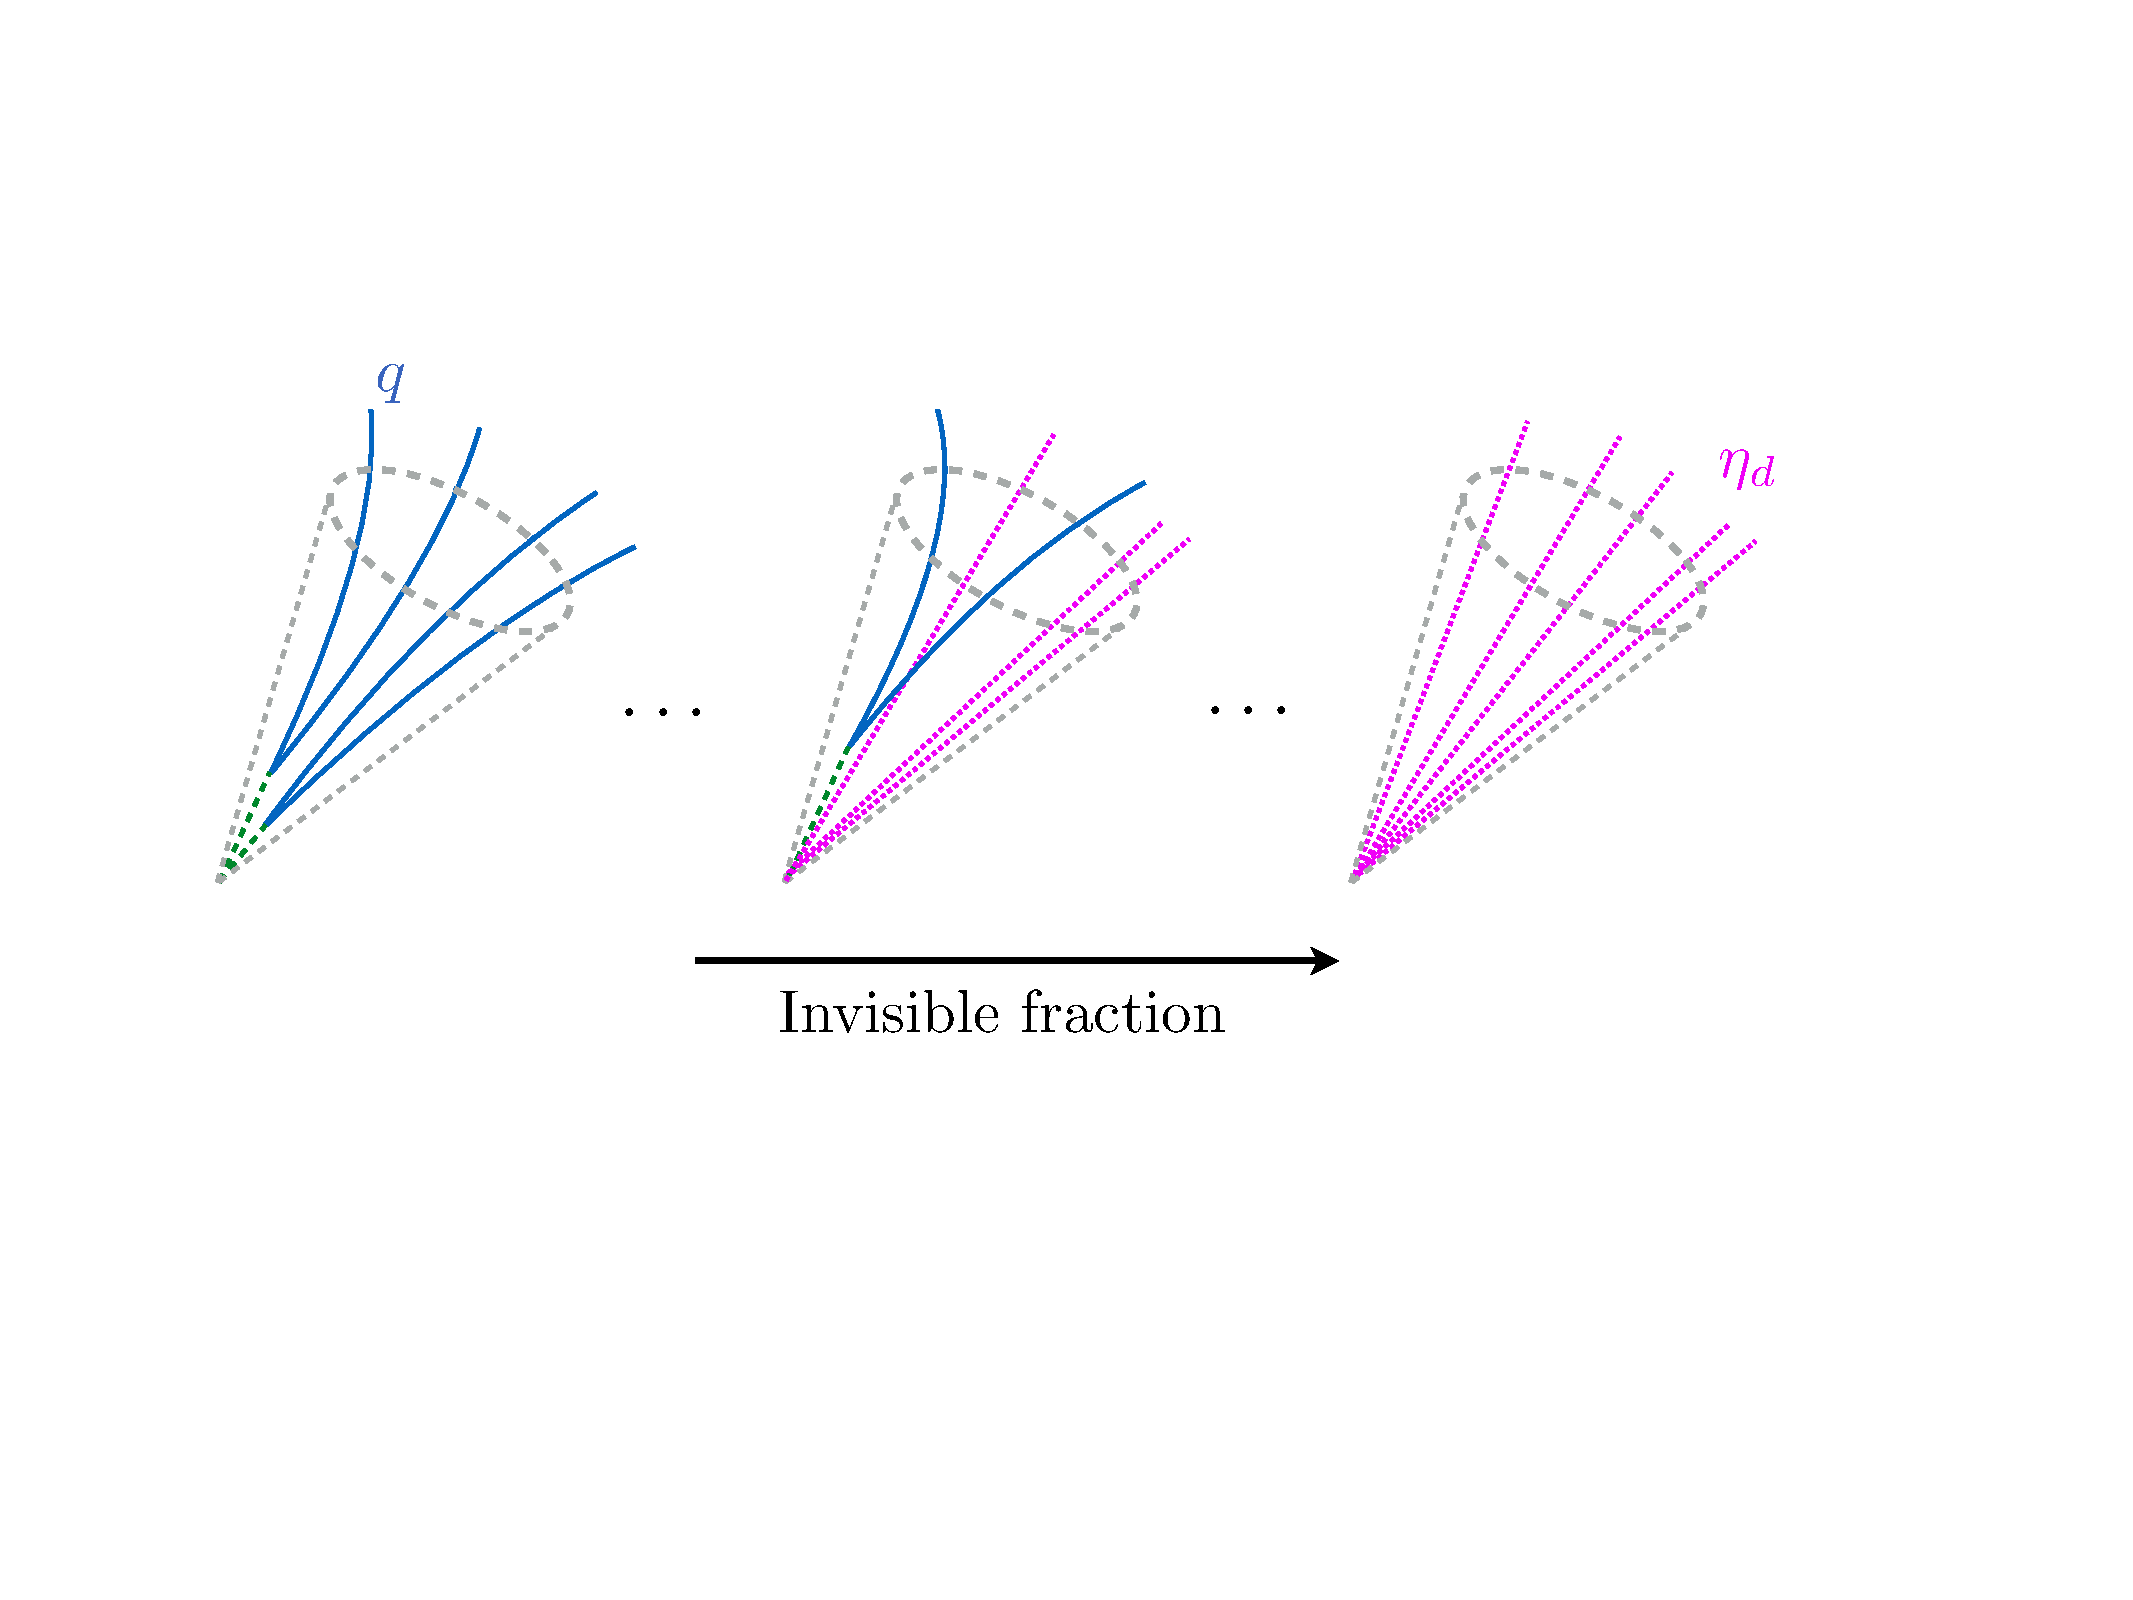
\includegraphics[width=0.75\textwidth]{figures/svj/r_inv.pdf}
\caption[The constituents of a semi-visible jet as a function of its invisible fraction]{The constituents of a semi-visible jet as a function of its invisible fraction \rinv \cite{Cohen:2017pzm}.}
\label{fig:theory_svj_rinv}
\end{figure}
